% !TEX program = xelatex
% ============================================================================
%  POSN Computer Qualification — Counting Slide Deck
%  Topic: การนับเบื้องต้น (Counting Principles)
% ============================================================================

\documentclass[11pt, aspectratio=169]{beamer}

% --- Load shared preamble ---
% ============================================================================
%  POSN Computer Qualification — Shared Beamer Preamble
%  Used by all topic slide decks. Compile with XeLaTeX.
% ============================================================================

% ---------- Thai language & font ----------
\usepackage{iftex}
\usepackage{fontspec}

% XeTeX-specific: enable Thai line breaking
\ifXeTeX
  \XeTeXlinebreaklocale{th}
\fi
% Noto Sans Thai — body text (clean modern sans-serif, handles all Thai)
\setmainfont{Noto Sans Thai}[
  UprightFont = Noto Sans Thai Light,
  BoldFont    = Noto Sans Thai Medium,
  Scale       = 0.9
]
\setsansfont{Noto Sans Thai}[
  UprightFont = Noto Sans Thai Light,
  BoldFont    = Noto Sans Thai Medium,
  Scale       = 0.9
]

% Noto Sans Thai — clean modern sans-serif for structural elements
\newfontfamily\headingfont{Noto Sans Thai}[
  UprightFont = Noto Sans Thai Medium,
  BoldFont    = Noto Sans Thai Bold,
  Scale       = 0.9
]

% --- Heading font for structural elements ---
\setbeamerfont{title}{family=\headingfont, series=\bfseries, size=\huge}
\setbeamerfont{subtitle}{family=\headingfont, series=\mdseries}
\setbeamerfont{author}{family=\headingfont, series=\mdseries}

% --- Custom Title Page ---
\defbeamertemplate{title page}{custom}[1][]{%
  \centering
  \vspace*{2cm}
  % Title — in white
  {\usebeamerfont{title}\color{white}\inserttitle\par}
  \vspace{0.6cm}
  % Subtitle — in white
  {\usebeamerfont{subtitle}\color{white}\insertsubtitle\par}
  \vspace{2.5cm}
  % Author — blue filled rounded box, white text
  \begin{center}
    \begin{tcolorbox}[arc=3mm, colback=boxBlue, colframe=boxBlue!80,
                      width=0.42\textwidth, halign=center,
                      left=1.5em, right=1.5em, top=0.8em, bottom=0.8em,
                      boxrule=1.5pt, coltext=white]
      \usebeamerfont{author}\insertauthor
    \end{tcolorbox}
  \end{center}
}
\setbeamertemplate{title page}[custom]
\setbeamerfont{frametitle}{family=\headingfont, series=\bfseries}
\setbeamerfont{section in toc}{family=\headingfont}
\setbeamerfont{page number in head/foot}{family=\headingfont}
\setbeamerfont{section title}{family=\headingfont, series=\bfseries}
\setbeamerfont{subsection title}{family=\headingfont}

% Monospace font (for code/verbatim)
\setmonofont{Latin Modern Mono}[Scale=0.9]

% ---------- Math ----------
\usepackage{amsmath, amssymb}

% ---------- Graphics ----------
\usepackage{graphicx}
\usepackage{tikz}

% ---------- String parsing (for section headers) ----------
\usepackage{xstring}

% ---------- Colored boxes ----------
\usepackage[skins, breakable, xparse]{tcolorbox}
% Note: we do NOT load the 'most' option — it predefines example/solution environments
% that would conflict with our custom boxes.

% --- Color definitions ---
\definecolor{boxBlue}{RGB}{41, 128, 185}
\definecolor{boxGreen}{RGB}{39, 174, 96}
\definecolor{boxOrange}{RGB}{230, 126, 34}
\definecolor{boxPurple}{RGB}{142, 68, 173}
\definecolor{boxBlueBg}{RGB}{235, 245, 255}
\definecolor{boxGreenBg}{RGB}{235, 255, 240}
\definecolor{boxOrangeBg}{RGB}{255, 245, 235}
\definecolor{boxPurpleBg}{RGB}{248, 240, 255}

% --- Explanation box (blue) — for definitions, concepts, notes ---
\newtcolorbox{explanation}[1][]{
  enhanced,
  breakable,
  arc         = 2mm,
  colback     = boxBlueBg,
  colframe    = boxBlue!50,
  title       = #1,
  fonttitle   = \bfseries\color{white},
  coltitle    = white,
  colbacktitle= boxBlue,
  attach boxed title to top left = {yshift=-2mm, xshift=2mm},
  boxed title style = {arc=2mm, size=small},
  before skip = 8pt,
  after skip  = 8pt
}

% --- Example box (green) — for worked examples ---
\newtcolorbox{exambox}[1][]{
  enhanced,
  breakable,
  arc         = 2mm,
  colback     = boxGreenBg,
  colframe    = boxGreen!50,
  title       = #1,
  fonttitle   = \bfseries\color{white},
  coltitle    = white,
  colbacktitle= boxGreen,
  attach boxed title to top left = {yshift=-2mm, xshift=2mm},
  boxed title style = {arc=2mm, size=small},
  before skip = 8pt,
  after skip  = 8pt
}

% --- Solution box (orange) — for solutions and answers ---
\newtcolorbox{solbox}[1][]{
  enhanced,
  breakable,
  arc         = 2mm,
  colback     = boxOrangeBg,
  colframe    = boxOrange!50,
  title       = #1,
  fonttitle   = \bfseries\color{white},
  coltitle    = white,
  colbacktitle= boxOrange,
  attach boxed title to top left = {yshift=-2mm, xshift=2mm},
  boxed title style = {arc=2mm, size=small},
  before skip = 8pt,
  after skip  = 8pt
}

% --- Intuition box (purple) — for plain-language explanations, analogies ---
\newtcolorbox{intuition}[1][]{
  enhanced,
  breakable,
  arc         = 2mm,
  colback     = boxPurpleBg,
  colframe    = boxPurple!50,
  title       = #1,
  fonttitle   = \bfseries\color{white},
  coltitle    = white,
  colbacktitle= boxPurple,
  attach boxed title to top left = {yshift=-2mm, xshift=2mm},
  boxed title style = {arc=2mm, size=small},
  before skip = 8pt,
  after skip  = 8pt
}

% ---------- Beamer theme ----------
\usetheme{Madrid}
\usecolortheme{default}

% --- Custom beamer colors (blue accent matching explanation boxes) ---
\setbeamercolor{structure}{fg=boxBlue}
\setbeamercolor{palette primary}{fg=white, bg=boxBlue}
\setbeamercolor{palette secondary}{fg=white, bg=boxBlue!80}
\setbeamercolor{palette tertiary}{fg=white, bg=boxBlue!60}
\setbeamercolor{block title}{fg=white, bg=boxBlue}
\setbeamercolor{block body}{fg=black, bg=boxBlueBg}

% Remove navigation symbols for clean look
\setbeamertemplate{navigation symbols}{}

% Note: Frame title prefix removed — \addtobeamertemplate conflicts with beamer internals

% --- Outline (Table of Contents) styling ---
\setbeamerfont{section in toc}{family=\headingfont, series=\mdseries}
\setbeamerfont{subsection in toc}{family=\headingfont, series=\mdseries}
\setbeamertemplate{section in toc}{%
  \leavevmode\leftskip=1.5em
  \textcolor{boxBlue}{\textbf{\large\inserttocsectionnumber.}}%
  \quad\inserttocsection\par
  \vspace{0.2em}
}
\setbeamertemplate{subsection in toc}{%
  \leavevmode\leftskip=4em
  \textcolor{boxBlue!60}{\small$\bullet$}%
  \quad\inserttocsubsection\par
  \vspace{0.1em}
}

% Section header slides — Thai in white, English in smaller light blue below
\AtBeginSection{
  \begin{frame}[plain]{}
    \vspace*{2cm}
    \begin{beamercolorbox}[sep=12pt, center, rounded=true, shadow=true]{palette primary}
      \IfSubStr{\secname}{(}{%
        \StrBefore{\secname}{(}[\sectionthai]%
        \StrBetween[1,1]{\secname}{(}{)}[\sectioneng]%
        \begin{tabular}{@{}c@{}}
          {\usebeamerfont{title}\sectionthai} \\[0.2em]
          {\usebeamerfont{subtitle}\color{boxBlue!60}\sectioneng}
        \end{tabular}%
      }{%
        {\usebeamerfont{title}\secname\par}%
      }
    \end{beamercolorbox}
    \vfill
  \end{frame}
}

% Subsection header slides — smaller, centered
\AtBeginSubsection{
  \begin{frame}[plain]{}
    \vfill
    \centering
    {\usebeamerfont{section title}\insertsubsectionhead\par}
    \vfill
  \end{frame}
}

% Minimal footer: page number only, right-aligned
\setbeamertemplate{footline}{
  \hfill\usebeamerfont{page number in head/foot}\insertframenumber{} / \inserttotalframenumber\hspace*{1em}\vspace*{0.5ex}
}

% ---------- Spacing & readability ----------
\linespread{1.2}

% ---------- Useful commands ----------

% Highlight important text in blue
\newcommand{\highlight}[1]{\textcolor{boxBlue}{\textbf{#1}}}

% Math set notation helpers
\newcommand{\R}{\mathbb{R}}
\newcommand{\N}{\mathbb{N}}
\newcommand{\Z}{\mathbb{Z}}
\newcommand{\Q}{\mathbb{Q}}

% ============================================================================
%  End of preamble
% ============================================================================


% --- Document info ---
\title[การนับ]{\textcolor{white}{การนับเบื้องต้น} \textcolor{boxBlue!60}{(Counting)}}
\subtitle{กฎการนับ • การเรียงสับเปลี่ยน • การจัดหมู่ }
\author[None W. (Yuan)]{None W. (Yuan)}
\date{}

\begin{document}

% ===========================================================================
%  TITLE SLIDE
% ===========================================================================
\begin{frame}[plain]
  \titlepage
\end{frame}

% ===========================================================================
%  OUTLINE
% ===========================================================================
\begin{frame}{สารบัญ (Outline)}
  \tableofcontents
\end{frame}

% ===========================================================================
%  ก่อนเรียน (Prerequisites)
% ===========================================================================
\begin{frame}{ก่อนเรียน (Prerequisites)}
  \begin{explanation}[สิ่งที่ควรรู้ก่อนเรียน]
    \begin{itemize}
      \item \textbf{เซต} — การดำเนินการของเซต, จำนวนสมาชิกของเซต
      \item \textbf{จำนวนเต็ม} — การคูณและการหาร, แฟกทอเรียล ($n!$)
    \end{itemize}
  \end{explanation}

  \begin{intuition}[หัวใจของการนับ]
    การนับเบื้องต้นคือ \highlight{การหาจำนวนวิธีทั้งหมด} ที่เหตุการณ์หนึ่งจะเกิดขึ้น
    โดยไม่ต้องนับทีละตัวอย่าง การนับมีประโยชน์ตั้งแต่การคำนวณความน่าจะเป็น
    ไปจนถึงการวิเคราะห์ขั้นตอนวิธี
  \end{intuition}
\end{frame}

% ===========================================================================
%  SECTION 1: หลักการนับเบื้องต้น (Basic Counting Principles)
% ===========================================================================
\section{หลักการนับเบื้องต้น}

\subsection{หลักการบวก (Addition Principle)}

\begin{frame}{หลักการบวก (Addition Principle)}
  \begin{explanation}[หลักการบวก]
    ถ้าต้องการทำงานอย่างหนึ่ง โดยสามารถเลือกทำได้จาก \highlight{กรณีที่แยกจากกัน}
    จำนวนวิธีทั้งหมด = \textbf{ผลรวม}ของจำนวนวิธีในแต่ละกรณี
  \end{explanation}

  \begin{exambox}[ตัวอย่าง: เลือกของว่าง]
    มีเค้ก 3 แบบ คุกกี้ 4 แบบ และขนมปัง 2 แบบ
    ถ้าต้องการเลือกขนมเพียง \textbf{1 ชิ้น} จะมีทั้งหมดกี่วิธี?

    \medskip
    \textbf{วิธีคิด:} เลือกเค้ก \textbf{หรือ} คุกกี้ \textbf{หรือ} ขนมปัง (คำว่า ``หรือ'' = บวก)
    \[
      3 + 4 + 2 = 9 \text{ วิธี}
    \]
  \end{exambox}

  \begin{intuition}[คิดง่าย ๆ]
    ``หรือ'' แปลว่า \highlight{บวก} — แต่ละกรณีแยกจากกัน ไม่ซ้อนทับกัน
  \end{intuition}
\end{frame}

\subsection{หลักการคูณ (Multiplication Principle)}

\begin{frame}{หลักการคูณ (Multiplication Principle)}
  \begin{explanation}[หลักการคูณ]
    ถ้าการทำงานประกอบด้วย \highlight{หลายขั้นตอนต่อเนื่องกัน} จำนวนวิธีทั้งหมด = \textbf{ผลคูณ}จำนวนวิธีในแต่ละขั้นตอน
  \end{explanation}

  \begin{exambox}[ตัวอย่าง: เลือกชุดเสื้อผ้า]
    มีเสื้อ 4 ตัว และกางเกง 3 ตัว
    จะแต่งตัวด้วยเสื้อ 1 ตัว \textbf{และ} กางเกง 1 ตัว ได้ทั้งหมดกี่แบบ?

    \medskip
    \textbf{วิธีคิด:} เลือกเสื้อ (4 วิธี) \textbf{และ} เลือกกางเกง (3 วิธี)
    \[
      4 \times 3 = 12 \text{ แบบ}
    \]
  \end{exambox}

  \begin{intuition}[คิดง่าย ๆ]
    ``และ'' แปลว่า \highlight{คูณ} — แต่ละขั้นตอนทำต่อเนื่องกัน
  \end{intuition}
\end{frame}

\begin{frame}[t]{ตัวอย่าง: การโยนเหรียญ (Coin Tossing)}
  \begin{exambox}[โจทย์]
    โยนเหรียญบาท 1 เหรียญ 3 ครั้ง
    จะมีผลลัพธ์ที่เป็นไปได้ทั้งหมดกี่แบบ?
  \end{exambox}

  \vspace{\fill}
\end{frame}

\begin{frame}[t]{ตัวอย่าง: การทอยลูกเต๋า (Dice Rolling)}
  \begin{exambox}[โจทย์]
    ทอยลูกเต๋า 1 ลูก 2 ครั้ง จงหา
    \begin{enumerate}
      \item[(ก)] จำนวนผลลัพธ์ทั้งหมด
      \item[(ข)] จำนวนวิธีที่ผลรวมของแต้มเป็นเลขคู่
    \end{enumerate}
  \end{exambox}

  \vspace{\fill}
\end{frame}

% ===========================================================================
%  SECTION 2: การเรียงสับเปลี่ยนเชิงเส้น (Linear Permutations)
% ===========================================================================
\section{การเรียงสับเปลี่ยนเชิงเส้น (Linear Permutation)}

\subsection{แฟกทอเรียลและนิยาม}

\begin{frame}{แฟกทอเรียล (Factorial)}
  \begin{explanation}[นิยาม: แฟกทอเรียล]
    สำหรับจำนวนเต็มบวก $n$,
    \[
      n! = n \times (n-1) \times (n-2) \times \cdots \times 2 \times 1
    \]
    ตัวอย่าง: $1! = 1, \;  2! = 2, \;  3! = 6, \;  4! = 24, \;  5! = 120$

    \medskip
    \textbf{นิยามเพิ่ม:} $0! = 1$
  \end{explanation}
\end{frame}

\begin{frame}{การเรียงสับเปลี่ยนเชิงเส้นคืออะไร?}
  \begin{explanation}[นิยาม: Permutation]
    \textbf{การเรียงสับเปลี่ยน} คือการจัดเรียงสิ่งของที่แตกต่างกันทั้งหมด
    โดย \highlight{คำนึงถึงลำดับ} (ลำดับต่าง = วิธีต่าง)
  \end{explanation}

  \begin{exambox}[ตัวอย่าง]
    จัดตัวอักษร A, B, C เรียงเป็นแถวตรง

    \medskip
    ตำแหน่งที่ 1: เลือกได้ 3 ตัว \quad $\rightarrow$ 3 วิธี

    ตำแหน่งที่ 2: เหลือ 2 ตัว \quad $\rightarrow$ 2 วิธี

    ตำแหน่งที่ 3: เหลือ 1 ตัว \quad $\rightarrow$ 1 วิธี

    \medskip
    จำนวนวิธีทั้งหมด = $3 \times 2 \times 1 = 3! = 6$ แบบ

    \medskip
    ได้แก่ ABC, ACB, BAC, BCA, CAB, CBA
  \end{exambox}
\end{frame}

\begin{frame}{สูตรการเรียงสับเปลี่ยน}
  \begin{explanation}[สูตร]
    \textbf{เลือกของ $r$ ชิ้นจาก $n$ ชิ้น เรียงลำดับ} (เรียกว่า $P(n, r)$):
    \[
      P(n, r) = \frac{n!}{(n-r)!}
    \]

    \medskip
    \textbf{เลือกของทั้งหมด $n$ ชิ้น เรียงลำดับ} (เรียงทุกตัว):
    \[
      P(n, n) = n!
    \]
  \end{explanation}
\end{frame}

\begin{frame}[t]{ตัวอย่าง: การเลือกกรรมการแบบมีตำแหน่ง}
  \begin{exambox}[โจทย์]
    มีคน 10 คน ต้องการเลือกกรรมการ 3 ตำแหน่ง (ประธาน, รองประธาน, เลขานุการ)
    โดยแต่ละคนดำรงตำแหน่งได้ตำแหน่งเดียว จะมีกี่วิธี?
  \end{exambox}

  \vspace{\fill}
\end{frame}

\begin{frame}[t]{ตัวอย่าง: ข้อสอบจริง}
  \begin{exambox}[โจทย์ปี 67 ข้อ 31]
    นักเรียนห้องหนึ่งมีชาย 3 คน หญิง 4 คนเรียงแถวถ่ายรูปโดยนักเรียนชายอยู่แถวหลัง นักเรียนหญิงอยู่แถวหน้าได้กี่วิธี
  \end{exambox}

  \vspace{\fill}
\end{frame}

% ===========================================================================
%  SECTION 3: การเรียงสับเปลี่ยนเชิงวงกลม (Circular Permutations)
% ===========================================================================
\section{การเรียงสับเปลี่ยนเชิงวงกลม (Circular Permutation)}

\begin{frame}{การเรียงสับเปลี่ยนเชิงวงกลมคืออะไร?}
  \begin{explanation}[แนวคิด]
    การจัดของ \highlight{รอบวงกลม} การหมุนวงกลมทั้งวง \textbf{ไม่ถือว่าเป็นวิธีที่ต่างกัน}
    เพราะตำแหน่งสัมพัทธ์ระหว่างสิ่งของยังคงเดิม
  \end{explanation}

  \begin{columns}[T]
    \column{0.45\textwidth}
      \centering
      \textbf{เส้นตรง: ลำดับต่าง = วิธีต่าง}

      \medskip
      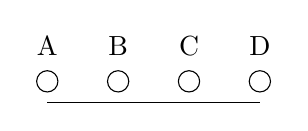
\begin{tikzpicture}[scale=0.9]
        \draw (0,0) circle (0.15) node[above=0.2cm] {A};
        \draw (1,0) circle (0.15) node[above=0.2cm] {B};
        \draw (2,0) circle (0.15) node[above=0.2cm] {C};
        \draw (3,0) circle (0.15) node[above=0.2cm] {D};
        \draw (0,-0.3) -- (3,-0.3);
      \end{tikzpicture}

      A-B-C-D $\neq$ B-C-D-A

    \column{0.45\textwidth}
      \centering
      \textbf{วงกลม: หมุนแล้วเหมือนเดิม}

      \medskip
      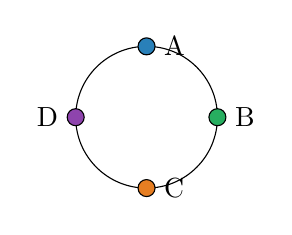
\begin{tikzpicture}[scale=0.9]
        \draw (0,0) circle (1);
        \draw[fill=boxBlue] (90:1) circle (0.12) node[right=0.1cm] {A};
        \draw[fill=boxGreen] (0:1) circle (0.12) node[right=0.1cm] {B};
        \draw[fill=boxOrange] (-90:1) circle (0.12) node[right=0.1cm] {C};
        \draw[fill=boxPurple] (180:1) circle (0.12) node[left=0.1cm] {D};
      \end{tikzpicture}

      หมุนแล้วได้รูปแบบเดิม
  \end{columns}
\end{frame}

\begin{frame}{สูตรการเรียงสับเปลี่ยนเชิงวงกลม}
  \begin{explanation}[สูตร]
    จำนวนวิธีจัดของ $n$ สิ่งที่แตกต่างกัน \textbf{รอบวงกลม}:
    \[
      (n-1)!
    \]

    \textbf{เหตุผล:} จัดของ $n$ สิ่งเป็นเส้นตรงได้ $n!$ วิธี
    แต่ละวิธีในวงกลมถูกนับซํ้า $n$ ครั้ง (จากการหมุน)
    ดังนั้น $\dfrac{n!}{n} = (n-1)!$
  \end{explanation}

  \begin{exambox}[ตัวอย่าง: จัดคนรอบโต๊ะกลม]
    จัดคน 5 คนนั่งรอบโต๊ะกลม จะนั่งได้ทั้งหมดกี่วิธี?

    \medskip
    \[
      (5-1)! = 4! = 24 \text{ วิธี}
    \]
  \end{exambox}
\end{frame}

\begin{frame}{กรณีพิเศษ: สร้อยคอหรือกำไล}
  \begin{explanation}[ข้อสังเกต]
    ถ้าวัตถุสามารถ \highlight{พลิกด้าน} ได้ (เช่น สร้อยคอ, กำไลข้อมือ)
    การพลิกด้านก็ไม่ถือว่าเป็นวิธีที่ต่างกัน
    จำนวนวิธีจะลดลงอีกครึ่งหนึ่ง:
    \[
      \frac{(n-1)!}{2}
    \]
  \end{explanation}

  \begin{exambox}[ตัวอย่าง: ร้อยลูกปัด]
    นำลูกปัด 6 สีที่แตกต่างกันมาร้อยเป็นสร้อยคอ จะได้สร้อยคอที่แตกต่างกันทั้งหมดกี่แบบ?

    \medskip
    \[
      \frac{(6-1)!}{2} = \frac{5!}{2} = \frac{120}{2} = 60 \text{ แบบ}
    \]
  \end{exambox}
\end{frame}

\begin{frame}{ทำไมสร้อยคอต้องหาร 2?}
  \begin{intuition}[การพลิกด้านของสร้อยคอ]
    ลองนึกถึงสร้อยคอ — ถ้าพลิกด้านกลับ หัวกลายเป็นท้าย
    แต่ลำดับของลูกปัดยังเหมือนเดิม (แค่มองจากอีกด้าน)

    \medskip
    ดังนั้น \highlight{ทุกแบบถูกนับซํ้า 2 ครั้ง} (ด้านหน้ากับด้านหลัง) จึงต้องหาร 2
  \end{intuition}

  \begin{explanation}[สรุปสูตร]
    \begin{itemize}
      \item จัดรอบวงกลม (พลิกไม่ได้ เช่น โต๊ะกลม): \quad $(n-1)!$
      \item จัดรอบวงกลม (พลิกได้ เช่น สร้อยคอ): \quad $\dfrac{(n-1)!}{2}$
    \end{itemize}
  \end{explanation}
\end{frame}

\begin{frame}[t]{ตัวอย่าง: ข้อสอบจริง}
  \begin{exambox}[โจทย์ปี 67 ข้อ 24]
    จำนวนวิธีในการจัดที่นั่งโต๊ะกลม เมื่อมีประธาน นักร้องวง A 4 คน และนักร้องวง B 3 คน และประธานต้องนั่งติดนักร้องทั้งสองวงมีกี่วิธี 
  \end{exambox}

  \vspace{\fill}
\end{frame}

% ===========================================================================
%  SECTION 4: การจัดหมู่ (Combinations)
% ===========================================================================
\section{การจัดหมู่ (Combination)}

\begin{frame}{การจัดหมู่คืออะไร?}
  \begin{explanation}[นิยาม: Combination]
    \textbf{การจัดหมู่} คือการเลือกสิ่งของ โดย \highlight{ไม่คำนึงถึงลำดับ}
    (ลำดับต่าง = วิธีเดียวกัน)
  \end{explanation}

  \begin{columns}[T]
    \column{0.45\textwidth}
      \centering
      \textbf{Permutation (ลำดับสำคัญ)}

      \medskip
      เลือก 2 คนจาก \{A, B, C\} เป็น\\
      ประธาน และ รองประธาน

      \medskip
      AB $\neq$ BA \\
      ได้ 6 วิธี = $P(3,2)$

    \column{0.45\textwidth}
      \centering
      \textbf{Combination (ลำดับไม่สำคัญ)}

      \medskip
      เลือก 2 คนจาก \{A, B, C\} เป็น\\
      กรรมการ (ตำแหน่งเดียวกัน)

      \medskip
      AB = BA \\
      ได้ 3 วิธี = $C(3,2)$
  \end{columns}
\end{frame}

\begin{frame}{สูตรการจัดหมู่}
  \begin{explanation}[สูตร]
    จำนวนวิธีเลือกของ $r$ ชิ้นจาก $n$ ชิ้น โดยไม่คำนึงถึงลำดับ:
    \[
      C(n, r) = \binom{n}{r} = \frac{n!}{r!(n-r)!}
    \]

    \medskip
    \textbf{ความสัมพันธ์กับ Permutation:}
    \[
      C(n, r) = \frac{P(n, r)}{r!}
    \]
    (เลือกมาก่อน $P(n,r)$ แล้วหารด้วยการสลับภายในกลุ่ม $r!$)
  \end{explanation}
\end{frame}

\begin{frame}[t]{ตัวอย่าง: การจัดหมู่}
  \begin{exambox}[โจทย์ 1]
    มีนักเรียน 10 คน ต้องการเลือกคณะกรรมการ 4 คน
    (ทุกคนมีตำแหน่งเท่ากัน) จะมีวิธีการเลือกกี่แบบ?
  \end{exambox}

  \vspace{\fill}
\end{frame}

\begin{frame}[t]{ตัวอย่าง: โยนเหรียญ}
  \begin{exambox}[โจทย์ 2]
    โยนเหรียญ 1 เหรียญ 5 ครั้ง จงหาจำนวนวิธีที่ได้หัว (H) 3 ครั้งพอดี
  \end{exambox}

  \vspace{\fill}
\end{frame}

\begin{frame}[t]{ตัวอย่าง: การเลือกไพ่}
  \begin{exambox}[โจทย์ 3]
    ในการเลือกไพ่ 2 ใบจากสำรับ 52 ใบ จะมีจำนวนวิธีทั้งหมดกี่วิธี?
  \end{exambox}

  \vspace{\fill}
\end{frame}

% ===========================================================================
%  SECTION 5: หลักการรังนกพิราบ (Pigeonhole Principle)
% ===========================================================================
\section{หลักการรังนกพิราบ (Pigeonhole Principle)}

\begin{frame}{หลักการรังนกพิราบ}
  \begin{explanation}[หลักการ]
    ถ้ามี \highlight{นก $n+1$ ตัว} บินเข้ารังนก \highlight{$n$ รัง}
    จะต้องมีอย่างน้อย \highlight{1 รัง} ที่มีนกอย่างน้อย \highlight{2 ตัว}
  \end{explanation}

  \begin{intuition}[คิดแบบบ้าน ๆ]
    ถ้ามีถุงเท้า 3 สีในลิ้นชัก แล้วคุณหลับตาหยิบ 4 ครั้ง
    ยังไงก็ต้องได้สีซํ้าอย่างน้อย 1 คู่แน่นอน
  \end{intuition}

  \begin{exambox}[ตัวอย่าง: วันเกิด]
    ในกลุ่มนักเรียน 13 คน
    จะต้องมีอย่างน้อย 2 คนที่เกิดเดือนเดียวกัน

    \textbf{เพราะ:} 1 ปีมี 12 เดือน (= 12 รัง) นักเรียน 13 คน (= นก 13 ตัว)
    $13 > 12$ จึงต้องมีเดือนที่มีนักเรียนอย่างน้อย 2 คน
  \end{exambox}
\end{frame}

\begin{frame}[t]{ตัวอย่าง: รังนกพิราบ}
  \begin{exambox}[โจทย์ 1]
    ในลิ้นชักมีถุงเท้า 3 สี (แดง, นํ้าเงิน, ดำ)
    อย่างละหลายคู่ ถ้าหลับตาหยิบถุงเท้าทีละข้าง
    ต้องหยิบอย่างน้อยกี่ข้างจึงจะมั่นใจว่าได้ถุงเท้าสีเดียวกัน 1 คู่?
  \end{exambox}

  \vspace{\fill}
\end{frame}

\begin{frame}[t]{ตัวอย่าง: ข้อสอบจริง}
  \begin{exambox}[โจทย์ปี 68 ข้อ 21]
    เลือกตัวเลขจากเซต $\{1, 2, 3, 4, 5, 6, 7\}$
    ต้องเลือกอย่างน้อยกี่จำนวนจึงจะมั่นใจว่ามี 2 จำนวนที่ผลรวมเป็น 8?
  \end{exambox}

  \vspace{\fill}
\end{frame}

% ===========================================================================
%  SUMMARY
% ===========================================================================
\section{สรุป}

\begin{frame}{สรุปเนื้อหา}
  \begin{explanation}[สิ่งที่ได้เรียนรู้]
    \begin{enumerate}
      \item \textbf{หลักการบวก}: ``หรือ'' — กรณีแยกจากกัน $\rightarrow$ \highlight{บวก}
      \item \textbf{หลักการคูณ}: ``และ'' — ขั้นตอนต่อเนื่อง $\rightarrow$ \highlight{คูณ}
      \item \textbf{Permutation}: เรียงลำดับ \quad $P(n,r) = \frac{n!}{(n-r)!}$
      \item \textbf{Circular Permutation}: จัดรอบวงกลม \quad $(n-1)!$
      \item \textbf{Combination}: ไม่เรียงลำดับ \quad $C(n,r) = \frac{n!}{r!(n-r)!}$
      \item \textbf{รังนกพิราบ}: นก $n+1$ ตัว $\rightarrow$ อย่างน้อย 1 รังมีนก $\geq 2$ ตัว
    \end{enumerate}
  \end{explanation}

  \begin{center}
    \large เอกสารนี้เป็นส่วนหนึ่งของเนื้อหาเตรียมสอบ \textbf{สอวน. คอมพิวเตอร์}
  \end{center}
\end{frame}

\end{document}
